\documentclass[runningheads]{llncs}

% \usepackage{epstopdf}
\usepackage{graphicx}
\usepackage{url}
\usepackage[breaklinks]{hyperref}
\usepackage{wrapfig}
\usepackage{supertabular}
\usepackage{algorithm}
\usepackage[noend]{algpseudocode}

\graphicspath{ {./images/} }

\hbadness=50000000
\vbadness=50000000

\hypersetup{
    colorlinks=true,
    linkcolor=blue,
    filecolor=magenta,
    urlcolor=cyan,
}

\begin{document}

\title{File Transfer Protocol Impremented in C}

\author{
    Adrian-Valentin Panaintescu
    \orcidID{0000-0002-5853-4764}
    }

\institute{
    Computer Science at the “Alexandru Ioan Cuza” University of Iasi
    }

\maketitle

\begin{abstract}
    The File Transfer Protocol (FTP) is a standard network protocol used for the transfer of computer files between a client and server on a computer network. The programs can be used on Unix-like operating systems.
    \keywords{File Transfer  \and Computer Network \and Unix}
\end{abstract}

\section{Introduction}
    This project is a server / client application that allows the transfer of computer files through the network. The server provides clients with a minimum number of commands that allow authentication, directory and file operation. Each user has managed permissions for each action they can take. User passwords are encrypted before being transmitted. There is a blocklist-based system to prevent malicious actions.
\section{The technologies used}
    The technologies involved in this project are TCP. The motivation for using this communication protocol is that TCP provides reliable, ordered, and error-checked delivery of a stream of bytes (bytes) between applications running on hosts communicating via an IP network and ensure data reception. \cite{w:tcp}

\section{Application architecture}
    The application is based on communication on a tcp protocol, server and clients. All files are stored on the server. After starting and configuring the server waits for the connection requests to come.

    \begin{figure}
        \centering
        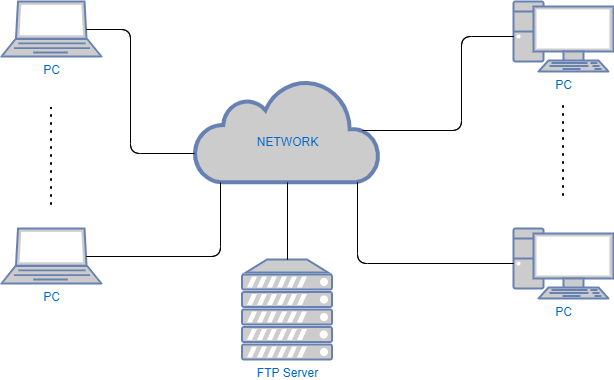
\includegraphics[width=0.8\textwidth,height=\textheight,keepaspectratio]{comunication}
        \caption{Communication between server and clients}
    \end{figure}

    When a connection request arrives and the connection is accepted, a child case process is created. It will take care of processing the commands received from the client.

    Communication between client and server is done through two sockets, one for control and one for the data that is created for each request.

    The client application at startup initializes the login process and waits for commands entered by the user on the keyboard. The entered command is initially processed by removing an int that speeds up the command id and its arguments. The command is sent with the argument. The server responded with a status code preceded by an action or ignoring that and returning to the stage of entering the command by the user.

\section{Implementation details}

    Communication is done through a dedicated socket for control. Orders are received and statuses are sent. The data exchange is performed on another socket, the data socket, which is created for each command. After processing orders it closes.

    The main features of this project is file sharing. This logic is shown in the diagram above.

    \begin{figure}
        \centering
        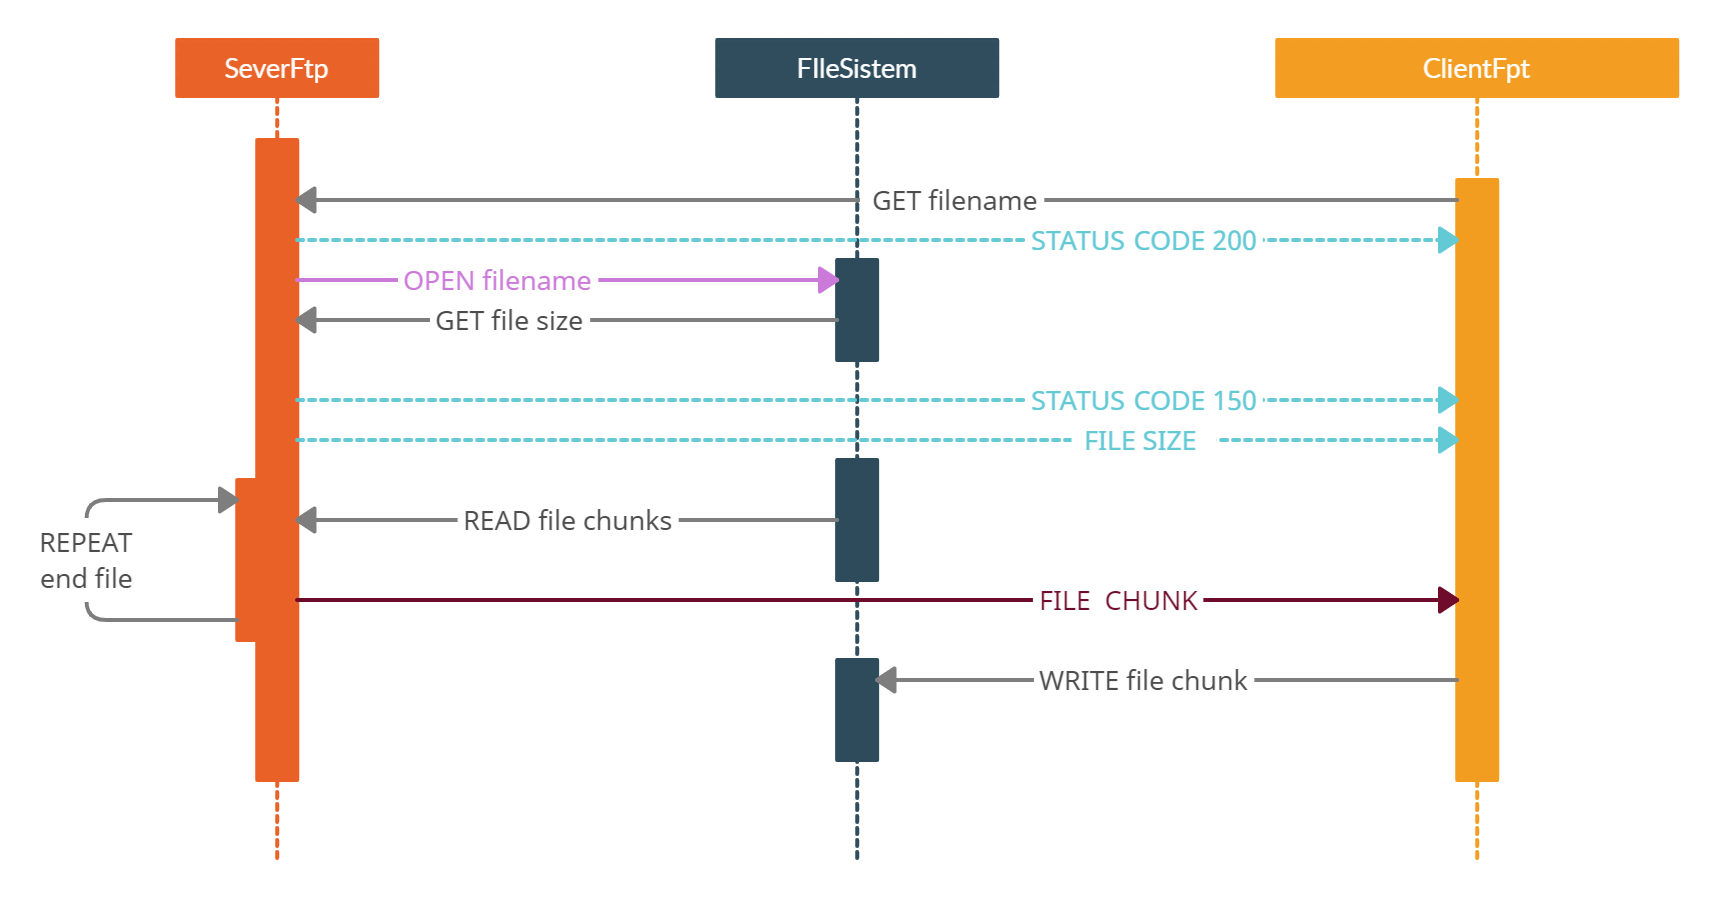
\includegraphics[width=0.9\textwidth,height=\textheight,keepaspectratio]{filesharing}
        \caption{File sharing comunication}
    \end{figure}

    \begin{algorithmic}[1]
        \State $config \gets readconfig()$
        \State $socket_{listen} \gets socketCreate(config["port"])$
        \While{$1$}
            \State $socket_{control} \gets socketAccept(socket_{listen})$
            \If{$fork()$}
                \State $close(socket_{listen})$
                \State $sendResponse(code_{ok})$
                \State $login()$
                \State $getPermision()$
                \While{$1$}
                    \State $r \gets reciveCommands()$
                    \State $r \gets checkPermision(r)$
                    \If{$ r = code_{ok} $}
                        \State $socket_{data} \gets socketConnect(socket_{control})$
                        \State $executeCommand()$
                        \State $close(socket_{data})$
                    \EndIf
                    
                    \If{$ r = code_{exit} $}
                        \State $break$
                    \EndIf
                    
                    \If{$ r = code_{unauthorized} $}
                        \State $contiune$
                    \EndIf
                    
                \EndWhile
                \State $close(socket_{control})$
            \State $a\gets b$
            \EndIf
            \State $close(socket_{control})$
        \EndWhile
        \State $close(socket_{listen})$
    \end{algorithmic}
    
    \subsection{Utilitarian Functions}
        A number of utilitarian functions are involved in both applications. These functions are found in a common file, together with which these two applications will be compiled. These functions are meant to shorten the length of the written code and to avoid duplicating the code.

        \subsubsection{int socket\textunderscore create(int port)}
            returns an open descriptor socket on the port provided as a parameter or -1 in case of error.
        \subsubsection{int socket\textunderscore accept(int sd)}
            returns a new socked descriptor about after the connection is accepted.
        \subsubsection{int socket\textunderscore connect(int port, char *host)}
            connect to remote host at given port and returns socket descriptor on success, -1 on error.
        \subsubsection{int recv\textunderscore data(int sockfd, char* buf, int bufsize)}
            receive data on sockfd. Returns -1 on error, number of bytes received on success.
        \subsubsection{int recv\textunderscore code(int sockfd)}
            receive a response from sockfd. Returns -1 on error, return code on success.
        \subsubsection{int send\textunderscore response(int sockfd, int rc)}
            send resposne code on sockfd. Returns -1 on error, 0 on success.
        \subsubsection{void print\textunderscore reply(int rc)}
            print the message for response code.
        \subsubsection{int file\textunderscore recive(int sock\textunderscore data, int sock\textunderscore control, char  path, int int s\textunderscore prog)}
            receive a file on sock\textunderscore data and save in path, comunicate with sock\textunderscore control. Return 0 on success, -1 on error.
        \subsubsection{int file\textunderscore send(int sock\textunderscore data, int sock\textunderscore control, char * path, int s\textunderscore prog)}
            send a file through sock\textunderscore data. Return 0 on succes, -1 on error.
        \subsubsection{void strtrim(char *str))}
            trim whiteshpace and line ending characters from string.
        \subsubsection{void strlow(char *str))}
            lower each string characters.
        \subsubsection{void read\textunderscore input(char * buffer, int size)}
            read input from command line.
        \subsubsection{int readconfig(char * dest, char * path, char * key)}
            copy key value on destination under the key in the file from path. Return bityes length copied.
        \subsubsection{void tree(char *basePath, const int root, FILE * file)}
            print in a file a tree view of base path.
        \subsubsection{void cripto(char * mess, char * key, int encoding)}
            encript mess with key. For each character$_i$ from is added to caracter$_i$ $\%$ key lenght if key is not 0 otherwise it decreases.
        \subsubsection{char * statkey(char * srt)}
            return a key based the string recived as parameter.
        \subsubsection{int is\textunderscore file(const char *path)}
            return 1 if it is a file else 0.
        \subsubsection{int remove\textunderscore directory(const char *path)}
            remove directory recursively. Return -1 on error.
        \subsubsection{int progressbar(long int p,long int t)}
            show progress bar
        \subsubsection{int filesize(char *path)}
            return filesize.
        


\section{Conclusions}
    The project illustrates the capability and advantages of a networked computer. I hope that the project will be enjoyed by a small group of people. Although it is insignificant compared to what software are launched on the market.

    For the future the application can be improved and add new features as well as added optimizations. Some tests must be done to determine how efficient the server is and to know what computational resources we need depending on the average number of clients and requests received per day / minute. In the client we can add functionalities for productivity or a text dye depending on the file format.
    \nocite{*}

\bibliographystyle{plainurl}
\bibliography{referinces}

\end{document}
